%! Author = anton
%! Date = 27/12/23

\documentclass[a4paper,12pt]{article}

% Required packages
\usepackage[utf8]{inputenc}  % UTF-8 encoding
\usepackage[T1]{fontenc}     % Font encoding
\usepackage{lmodern}         % Modern font
\usepackage{geometry}        % To adjust the page margins
\geometry{margin=0.9in}      % 0.9 inch margins

\usepackage{algorithm}       % Algorithms
\usepackage{algorithmic}     

\usepackage{amsmath}         % Advanced math symbols
\usepackage{graphicx}        % To include images
\usepackage{hyperref}        % For hyperlinks
\usepackage{float}           % For images

\usepackage[normalem]{ulem}  % Tables
\useunder{\uline}{\ul}{}
\usepackage{booktabs}
\usepackage{rotating}
\usepackage{array}
\usepackage{colortbl}   % For coloring table rows
\usepackage{xcolor}     % For color definitions
\usepackage{caption}    % For customizing captions


% Title information
\title{Solving the K Knights Problem with Backtracking}
\author{Antonio Bruno}
\date{\today}

\begin{document}

% Generate the title
\maketitle

% Beginning of the content
\section{Introduction}
This report presents a solution to the \( k \) knights problem using \textbf{Constraint Satisfaction Problem (CSP)} techniques; in particular,
we will refer to exercise 6.2 of the book "Artificial Intelligence: A Modern Approach" by Stuart Russell and Peter Norvig (Third Edition).
The problem consists of placing \( k \) knights on an \( n \times n \) chessboard such that no knight attacks another knight. The goal is to efficiently find a solution to the problem and visualize it using a graphical interface.
The solver algorithm is implemented in Python and is based on the \textbf{backtracking} search algorithm with \textbf{Maintaining Arc Consistency (MAC)} and 
several heuristics to improve the search efficiency. The graphical interface is implemented using the Matplotlib library to display 
the chessboard. 

If you are interested in the code, you can find it in the \href{https://github.com/antnatb/k-knights}{GitHub repository}.

\section{Problem Description}
The knights problem is a classic puzzle that involves placing knights on a chessboard in such a way that no two knights can threaten
each other. The chessboard is an \( n \times n \) grid, and a knight can move in an L-shape: two squares in one direction and then
one square perpendicular, or one square in one direction and then two squares perpendicular.

The specific problem addressed in this project is to determine how to place \( k \) knights on an \( n \times n \) chessboard
so that no two knights threaten each other, where \( k \) is given and is less than \( n^2 \). The goal is to find a valid configuration or to determine
that no such configuration exists.

While finding a solution to this problem may initially seem challenging, there is a straightforward approach. When a knight moves, it always lands on a square of the opposite color from where it started (e.g., if it starts on a white square, it lands on a black square, and vice versa). Consequently, if all knights are placed on squares of the same color, no knights will threaten each other. By positioning the knights in this manner, a solution is guaranteed for any given \(k\). The maximum value of knights that can be placed without threats corresponds indeed the maximum number of cells of the one color on the chessboard, i.e. \( n^2 / 2\) if \( n\) is even or \( {(n^2 + 1)} / 2\) if \(n\) is odd.

\section{Methodology and Implementation}
The problem is modeled as a Constraint Satisfaction Problem and solved using a backtracking search algorithm with Maintaining 
Arc Consistency (MAC). A CSP is characterized by a set of \textbf{variables}, a set of \textbf{domains} (one for each variable), and a set of \textbf{constraints} that
define the relationships between the variables. Backtracking search is a general algorithm for finding solutions to CSPs by systematically exploring the 
search space and backtracking when a constraint violation is detected. MAC is a technique that enforces arc consistency on the
constraints of the problem, reducing the search space and improving the efficiency of the search; in particular, inference
is done through the \textbf{AC-3} algorithm. For details about the mentioned algorithms, see sections 6.2 and 6.3 of R\&N 2021.

I decided to model the problem in two different ways:
\begin{itemize}
    \item \textbf{Implementation 1:} the variables are the positions of the \( k \) knights on the board and consequently the domain of each variable is the set of all possible squares on the chessboard. Every variable has a binary constraint with each other variable because every knight is potentially threatened by each other one; naturally the constraint \textit{allDiff} is present, because two knights cannot be placed on the same square
    
    \item \textbf{Implementation 2:} the variables are all the squares on the chessboard and their domain is $\{0; 1\}$: 1 if there's a knight and 0 otherwise. Here, there are binary constraints between squares that constitute a threat (they can't be both equal to 1 simultaneously), and there is a global constraint as well: the sum of all assigned values must be equal to \( k \), that is there must be \( k \) knights placed on the board. 
\end{itemize}

While both implementations share a significant portion of the problem structure and solving techniques, they exhibit some notable differences:
\begin{itemize}
    \item \textbf{Number of possible assignments:} Due to differing variables and domains, the two implementations have distinct sizes for their respective sets of possible assignments. In particular, implementation 1 has \(k\) variables with \(|D_i|=n^2\), resulting in at most \(n^{2k}\) possible assignments (not considering any constraints), whereas implementation 2 has at most \(2^{n^2}\) possible assignments, since there are \(n^2\) variables and \(|D_i|=2\). They are both very large numbers but the first one is in most cases relatively bigger, even though inferences and constraints reduce these numbers significantly.
    \item \textbf{Inference:} In implementation 2, \textbf{arc-consistency} has no need to propagate during AC-3, as the domain of revised variables can only be reduced to {0}, and 0 will always be a consistent value if we consider binary constraints only. For this reason, AC-3 does not propagate the inference to revised variables and cannot return False either, but it's still useful to maintain arc consistency. On the contrary, in implementation 1 AC-3 is more efficient and has the ability of determining if a current assignment cannot lead to a solution.
    \item \textbf{Choice of variable:} when choosing which variable to assign, both implementations make use of the \textbf{Minimum Remaining Values (MRV)} heuristic, i.e, the variable with the smallest domain is chosen in order to obtain a fail-first search. However, in the case of implementation 2, the set of variables is initially shuffled, in order to avoid having the same (and inefficient) search tree on every execution of the algorithm.
    \item \textbf{Choice of value:} when choosing which value to assign first to any variable, different techniques are used in each implementation. In implementation 1, the \textbf{Least Constraining Value} heuristic is used, i.e. the value which leaves more options for other variables is chosen, increasing the chances of finding a solution if there is one. In implementation 2, the value 1 is always chosen first, because we want to try and place a knight whenever we can.
    \item \textbf{Global constraints:} global constraints are treated differently: in implementation 1, the constraint is directly treated during AC-3, labeling two knights being on the same square as a threat and thus considering the case when checking for arc-consistency. In implementation 2, the global constraint is checked when choosing the next variable to assign; if the number of placed knights plus the number of unassigned squares is less than \(k\), then no solution is possible with the current placement, so the search can be pruned.
\end{itemize}

These differences produce some interesting results in the efficiency of the solver algorithms, which we will discuss in the following section.

\section{Results} \label{sec:Results}
Both implementations successfully find a solution to the \(k\) knights problem if one exists, or return None if no solution is possible (figure \ref{fig:solutions}). However, depending on the problem size, the execution time can be relatively long.

\begin{figure}[H]
    \centering
    \begin{minipage}{0.45\textwidth}
        \centering
        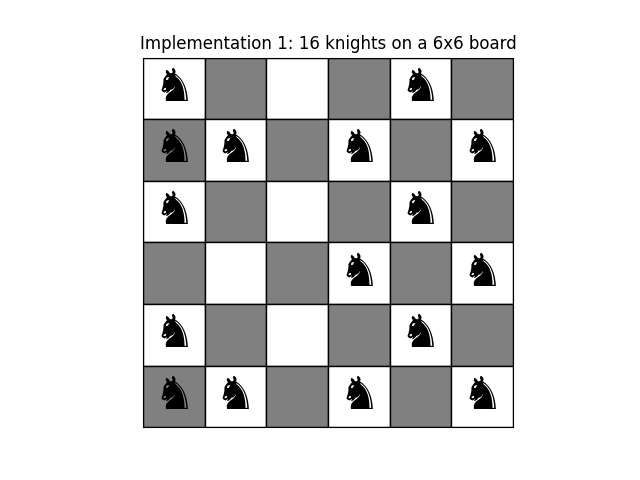
\includegraphics[width = \textwidth]{images/im1_k16_n6.png}
    \end{minipage}
    \hfill
    \begin{minipage}{0.45\textwidth}
        \centering
        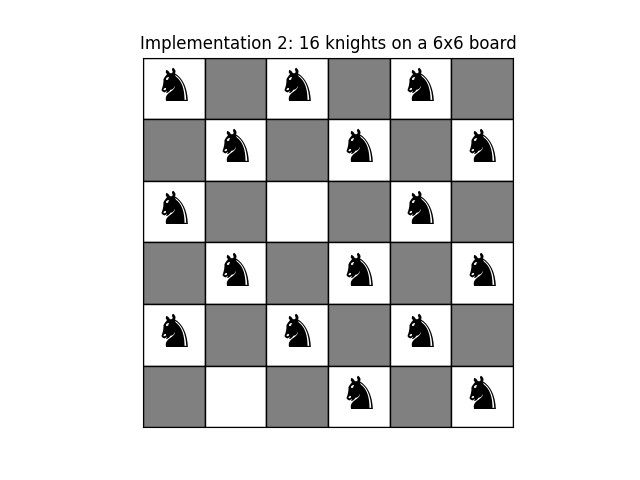
\includegraphics[width = \textwidth]{images/im2_k16_n6.png}
    \end{minipage}
    \caption{The solutions found by implementation 1 (left) and implementation 2 (right) to a problem with \(k = 16\) and \(n = 6\)}.
    \label{fig:solutions}
\end{figure}


Implementation 1 consistently returns the same result for a given input, maintaining consistent execution times for fixed values of \(n\) and \(k\). When \(k\) is less than or equal to a critical threshold value (which we will call \textbf{c} for a given n, the execution time is relatively small. However, beyond this critical value, the execution time increases dramatically. Consequently, when attempting to place the maximum number of knights on an n × n chessboard, Implementation 1 often takes too long, making Implementation 2 a more viable option in these cases.

On the other hand, Implementation 2 finds different solutions each time it runs and does not exhibit the same critical threshold behavior as Implementation 1. However, for values of k below the critical threshold of Implementation 1, the average execution time of Implementation 2 is longer than that of Implementation 1. This makes Implementation 1 more efficient for smaller problem sizes within the threshold, while Implementation 2 is preferable for larger problem sizes or when the maximum number of knights needs to be placed.

I have run multiple tests in order to individuate the critical value \textbf{c} for a given n and test the general running times of the algorithms, and the results are shown in the following table, where \textbf{t1(s)} is the time taken on the given problem by implementation 1 and \textbf{t2(s)} is the average time taken (on 3 measurements) by implementation 2: 

\begin{table}[H]
    \centering
    \begin{tabular}{l|c|c|c|c|c|c|c|c|c|c|}
        \textbf{n} & 6 & 7 & 8 & 9 & 10 & 11 & 12 & 13 & 14 & 15 \\
        \textbf{c} & 16 & 25 & 26 & 41 & 42 & 51 & 62 & 72 & 87 & 98 \\
        \textbf{t1(s)} & 0.03 & 0.14 & 0.27 & 1.05 & 1.53 & 3.27 & 7.14 & 13.43 & 27.01 & 44.54 \\
        \textbf{t2(s)} & 0.02 & 0.10 & 1.50 & \underline{49.70} & \underline{165.2} & \underline{638.4} & \underline{8234.2} & ... & ... & ... \\
    \end{tabular}
    \caption{Results of the tests: \(c\) knights on a \(n\times n\) chessboard, where \(c\) is the critical value for implementation 1}
    \label{tab:results}
\end{table}

As you can see, the running time of implementation 2 skyrockets when \(n>8\). In general, for chessboards of size \(n \times n\) with \(n <= 8\), implementation 2 is  more efficient for every possible \(k\) and is indeed preferable for values of \(k>c\); however for \(n>8\) implementation 2 becomes significantly less efficient and implementation 1 is favorable if \(k<=c\). It is to be noted that since implementation 2 explores a random search tree on every execution, it may be possible with some luck to find a solution in relatively small time for larger inputs; for the same reason, if you reproduce the test it is possible and likely to obtain different running times from the ones shown in the table, since the number of measurements is relatively small.


\section{Conclusion}
In conclusion, the \(k\) knights problem can be solved using Constraint Satisfaction Problem techniques and backtracking search algorithms, 
but it's not the most efficient approach for large values of \( k \) and \( n \); it's likely that the use of different and combined heuristics
and inference techniques will improve the efficiency of the search and reduce the time complexity of the algorithm. 

A simple and straightforward algorithm for this exact problem would be the following:

\begin{algorithm}
    \caption{Algorithm to place knights on a chessboard}
    \label{algo:knight_placement}
    \begin{algorithmic}[1]
        \STATE \textbf{Input:} An \( n \times n \) chessboard and \( k \) knights
        \STATE \textbf{Output:} A valid configuration of knights on the board
        \IF {$k > \lceil \frac{n^2}{2} \rceil $}
            \STATE \textbf{return} "No solution exists"
        \ELSE
            \STATE Place the first knight in the top-left corner of the board
            \IF {the top-left corner of the board is white}
                \STATE place all other knights on white squares
            \ELSE 
                \STATE place all other knights on black squares
            \ENDIF
            \STATE \textbf{return} "Solution found"
        \ENDIF
    \end{algorithmic}
\end{algorithm}

This algorithm is guaranteed to find a solution if one exists and it is as efficient as possible, with a time complexity of \( O(k) \).

% End of the content
\end{document}

